\chapter{Preliminaries}\label{ch:preliminaries}

In this chpater, 

\section{SpecElicitor}

SpecElicitor is a tool made by Yuan-Hong Lo, 
which can help user testing Mobile Application with friendly GUI interface.

When user start using SpecElicitor,
each time user do an action, such as clicking a button, on the Mobile Application, 
the tool will ask for labeling the action and the screen shown on the interface.
By using SpecElicitor, we can choose the specified action at every step, label the meaning of the action,
and label the exception situation if it happen and stop the trace at any time we need.
The interface of the SpecElicitor is shown in Fig[\ref{SpecElicitorInterface}].


The traces made by SpecElicitor include automata, screenshots, XML files and labels.
The automata is a json file record every states and edges on the traces.
A state has a screenshot and a XML file dumped from the Mobile,
and an edge records the action user did such as clicking element, typing text or exiting the Application.
The traces also record labels on every states and edges,
so we can recognize how many label we focus on happened on the trace.
An example trace of Recipe Application made by SpecElicitor is shown in Fig[\ref{SpecElicitorTraces}].

%Our LAb 建立了一個工具SpecElicitor
%使用者可以在GUI介面下一邊建立APP的trace, 同時標記該畫面/動作的label
%使用完後會產生含有 XML, 截圖, label的traces

\begin{figure}[ht]
	\graphicspath{{pic/}}
	\begin{center}
		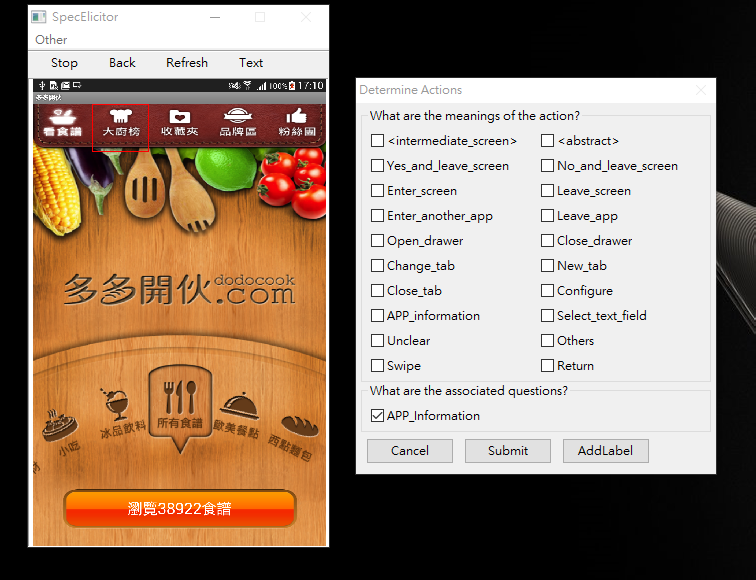
\includegraphics[width=0.8\textwidth]{SpecElicitorInterface.png}
		\caption{ The GUI interface of SpecElicitor.  }
		\label{SpecElicitorInterface}
	\end{center}
\end{figure}

\begin{figure}[ht]
	\graphicspath{{pic/}}
	\begin{center}
		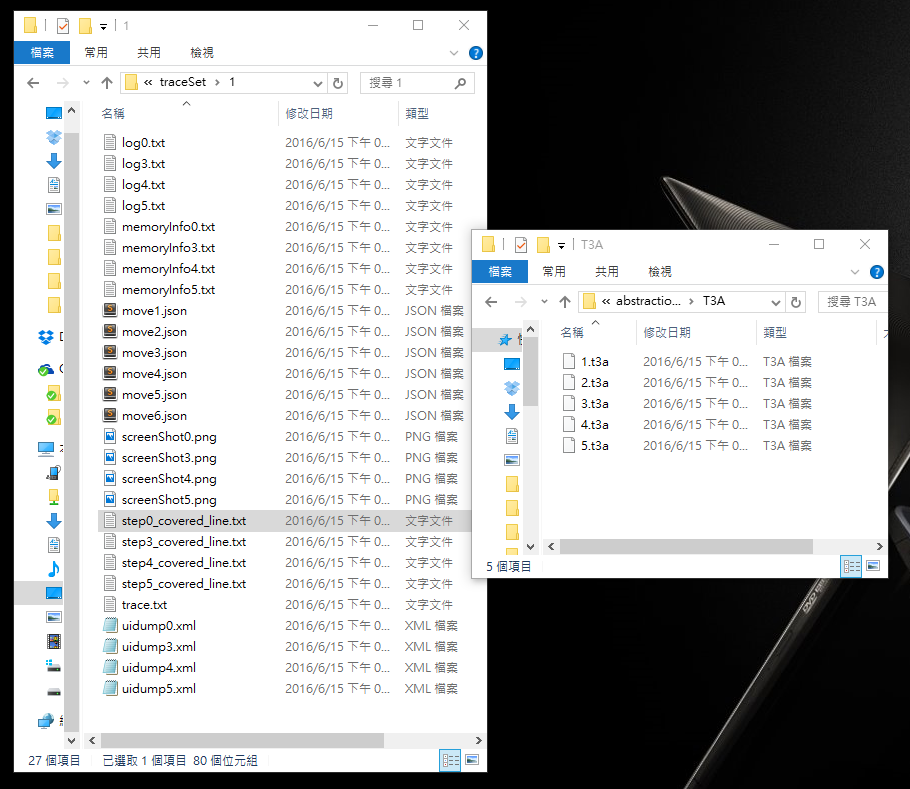
\includegraphics[width=0.8\textwidth]{SpecElicitorTraces.png}
		\caption{ An example of the traces.  }
		\label{SpecElicitorTraces}
	\end{center}
\end{figure}

\clearpage

\section{Common Sense Label}

We construct a label dictionary of common sense, which represents the behaviors of applications.
There are different kinds of applications, however,
people will expect that same kind of applications perform the similar behaviors and generate similar results.
By generalizing those similar applications with behaviors,
we transform the behaviors of applications into the common sense model and use normalized terms to represent the common sense.

The label dictionary collects normalized terms from several kinds of applications.
A common sense, defined as a normalized term, represent a concept of a screen shown on the platform or an action for a clicking event.
For instance, the label dictionary of File Manager application is listed in Table \ref{LabelDictionaryTable}.
Take file manager as example, the button "REMOVE" and "DELETE" represent the same concept of behavior, removing the selected file.
People except this two buttons have same performance when people use in two different file manager applications.
We define this concept of action and represented by a normalized term "delete-file".
With the help of label dictionary,
the trace of different appliactions, which consist of screens and actions, 
can represent by list of common sense label.


\begin{table}[ht]
	\begin{center}
		\begin{tabular}{ l | l }
			\hline
			Screen labels & Action labels \\
			\hline\hline
			Folder & Change-folder \\
			Create-query & Open-file \\
			Search-Query & Create-file \\
			Compress-query & Creare-folder \\
			Delete-query & Search-file-or-forder \\
			Rename-query & Select-all \\
			Copy-query & Select-file-or-folder \\
			Cut-query & Deselect \\
			Paste-query & Compress-file-or-folder \\
			Move-query & Delete-file-or-folder \\
			Bookmark-screen & Rename-file-or-folder \\
			Item-information & Copy-file-or-folder \\
			  & Cut-file-or-folder \\
			  & Paste-file-or-folder \\
			  & Move-file-or-folder \\
			  & Refresh \\
			
			%{1-2}
			%\multicolumn{2}{c|}{ dd }  \\
			%\cline{1-2}
		\end{tabular}
		\caption{ Common sense labels of File Manager Application.  }
		\label{LabelDictionaryTable}
	\end{center}
\end{table}

%將APP建立出state-base的automata,其中screen作為state,action作為edge
%用統一的normalized terms來specific
%our Lab建立一個TAAD的SpecElicitor,可產生label的trace

\clearpage

\section{Support Vector Machine}

Machine learning is widely used in recognition and classification problems.
For example, handwriting recognition can predict the letter without using keyboard.
Generally, the dataset used by machine learning would be divided into training set and testing set.
the training set would be analyzed and used to construct a model,
which can make prediction on the testing set.

In our work, we use the Support Vector Machine as our machine learning algorithm to solve the classification problem of traces.
Support Vector Machine is a well-known algorithm in machine learning and widely used for classification and regression analysis.
SVM is a supervised learning algorithm and it needs the training data labeled.
SVM find a hyper-plane in a high dimensional space in order to seperate the instances
The optimal hyper plane has the largest margin, which means the distance between the hyper plane and the closest trainging data. 

We collect the testing traces from web and mobile applications.
Because each instances in the data set should be formalized to a set of feature vector,
We use the label dictionary mentioned above as the featuer vector and transform the traces to vectors consist of label features.
In order to evaluate traces, we train the SVM with the labeled traces.
Then we can predict unlabeled traces and classify them into passed traces and failed traces.



%svm 在高維度 用largest margin來 seperate datas 
%svm可用來 cluster data

